\documentclass[12pt,a4paper]{article}
\usepackage{amsmath,amsthm,amssymb,mathtools}
\usepackage{tikz}
\usetikzlibrary{arrows.meta,positioning,shapes.geometric,calc,fit,backgrounds}
\usepackage{graphicx}
\usepackage{booktabs,tabularx,multirow}
\usepackage[ruled,vlined,linesnumbered]{algorithm2e}
\usepackage[most]{tcolorbox}
\usepackage{hyperref}
\usepackage[capitalize,noabbrev]{cleveref}
\usepackage[margin=1in]{geometry}
\usepackage{fancyhdr}
\usepackage{enumitem}
\usepackage{xcolor}

%% tcolorbox environments
\newtcolorbox{keyinsight}[1][]{colback=blue!5!white,colframe=blue!75!black,fonttitle=\bfseries,title=Key Insight,#1}
\newtcolorbox{example}[1][]{colback=green!5!white,colframe=green!75!black,fonttitle=\bfseries,title=Example,#1}
\newtcolorbox{warningbox}[1][]{colback=red!5!white,colframe=red!75!black,fonttitle=\bfseries,title=Warning,#1}

%% amsthm environments
\newtheorem{theorem}{Theorem}[section]
\newtheorem{lemma}[theorem]{Lemma}
\newtheorem{definition}{Definition}[section]
\newtheorem{remark}{Remark}[section]

%% Header / footer
\pagestyle{fancy}
\fancyhf{}
\rhead{Deep Learning -- Session 11}
\lhead{IIIT Dharwad}
\cfoot{\thepage}

%% Colour shortcuts
\definecolor{codeblue}{RGB}{0,0,180}
\definecolor{codegray}{RGB}{128,128,128}
\definecolor{pyorange}{RGB}{220,100,0}

\hypersetup{
  colorlinks=true,
  linkcolor=blue!60!black,
  urlcolor=blue!60!black,
  citecolor=green!50!black
}

\title{%
  \vspace{-1cm}
  {\Large Deep Learning -- Session 11}\\[6pt]
  {\LARGE \textbf{PyTorch Dataset \& DataLoader Abstraction\\
  and ANN Hands-On with Fashion-MNIST}}\\[8pt]
  {\large Lecture Notes}
}
\author{%
  Prof.\ S R M Prasanna \quad \& \quad Dr.\ Sunil Saumya\\[4pt]
  \normalsize Indian Institute of Information Technology Dharwad
}
\date{Session 11 \quad $\cdot$ \quad Duration: $\approx 2$h 01m}

\begin{document}

\maketitle
\thispagestyle{fancy}

\begin{abstract}
This document presents comprehensive lecture notes for Session~11 of the Deep
Learning course at IIIT Dharwad.  The session is a hands-on implementation
class covering two tightly coupled topics: (1)~PyTorch's \texttt{Dataset} and
\texttt{DataLoader} abstractions that decouple data definition from batch
iteration, and (2)~the end-to-end construction, training, and evaluation of a
three-layer Artificial Neural Network (ANN) on the Fashion-MNIST dataset.  The
document reproduces all slide content, code walkthroughs, parameter-count
derivations, and Q\&A discussions that occurred during the live session.
\end{abstract}

\tableofcontents
\newpage

%% ============================================================
\section{Introduction and Session Overview}
\label{sec:intro}
%% ============================================================

Session~11 marks the transition from conceptual understanding of neural
networks to full PyTorch implementation.  The instructor (Prof.\ Prasanna)
opens with a brief recap of the previous class, which introduced greedy
layer-wise unsupervised pre-training as practised circa 2006, and then pivots
to a wholly hands-on agenda.

\begin{keyinsight}
The central pedagogical goal of Session~11 is to show students a
\emph{complete} deep-learning pipeline in PyTorch: loading raw CSV pixel data,
wrapping it in a custom \texttt{Dataset}, batching it with \texttt{DataLoader},
defining a network as an \texttt{nn.Module} subclass, running the training
loop, and evaluating classification accuracy -- all for a real benchmark
dataset (Fashion-MNIST).
\end{keyinsight}

\subsection{Agenda}

\begin{enumerate}[label=\arabic*.]
  \item Recap of previous session (greedy layer-wise training, \texttt{nn.Module} introduction).
  \item PyTorch \texttt{Dataset} abstraction -- motivation and three required methods.
  \item \texttt{DataLoader} -- batching, shuffling, and iteration protocol.
  \item Fashion-MNIST dataset overview.
  \item ANN architecture design: $784 \to 128 \to 64 \to 10$.
  \item Hands-on Colab walkthrough: data loading, preprocessing, model definition, training loop, evaluation.
  \item \texttt{torchinfo} model summary and parameter count verification.
\end{enumerate}

\subsection{Prerequisites}

Students are expected to be familiar with:
\begin{itemize}
  \item Python object-oriented programming (classes, constructors, inheritance).
  \item PyTorch tensors and basic \texttt{nn.Module} usage (introduced in Session~10).
  \item Forward propagation, loss functions, and back-propagation (covered in earlier sessions).
  \item Stochastic Gradient Descent and the concept of mini-batch training.
\end{itemize}

%% ============================================================
\section{Background and Prerequisites}
\label{sec:background}
%% ============================================================

\subsection{Why Abstractions Are Needed}

Raw data arrives in many forms -- CSV files, image folders, HDF5 archives,
database tables.  A neural network, however, requires a \emph{tensor} as
input.  Without a principled abstraction layer, every project requires custom
glue code that intermixes data-loading logic with training logic.  PyTorch
solves this with two clean abstractions:

\begin{itemize}
  \item \texttt{torch.utils.data.Dataset} -- defines \emph{what} the data is
        and \emph{how} to access a single sample.
  \item \texttt{torch.utils.data.DataLoader} -- defines \emph{how} to iterate
        over the dataset in mini-batches.
\end{itemize}

\begin{definition}[Separation of Concerns in Data Loading]
\label{def:separation}
The \emph{Dataset--DataLoader} pattern enforces a clean separation:
\begin{align}
  \texttt{Dataset} &\;\longleftrightarrow\; \text{``what is a single sample?''} \notag \\
  \texttt{DataLoader} &\;\longleftrightarrow\; \text{``how do I iterate efficiently over many samples?''} \notag
\end{align}
\end{definition}

\subsection{Object-Oriented Programming Refresher}

Both \texttt{Dataset} and \texttt{nn.Module} are \emph{abstract base classes}
that students subclass to provide concrete behaviour.  Key OOP concepts
relevant to this session are summarised in \cref{tab:oop}.

\begin{table}[htbp]
  \centering
  \caption{OOP concepts used in Session~11}
  \label{tab:oop}
  \begin{tabularx}{\linewidth}{lX}
    \toprule
    \textbf{Concept} & \textbf{Role in this session} \\
    \midrule
    Class & Blueprint for \texttt{CustomDataset}, \texttt{MyNN} \\
    Object (instance) & \texttt{train\_dataset}, \texttt{model}, \texttt{optimizer} \\
    Constructor (\texttt{\_\_init\_\_}) & Runs automatically when an object is created; used to load data or define layers \\
    Inheritance & \texttt{CustomDataset(Dataset)}, \texttt{MyNN(nn.Module)} inherit parent behaviour \\
    \texttt{super().\_\_init\_\_()} & Calls the parent class constructor to initialise inherited attributes \\
    Method override & Subclass provides concrete \texttt{\_\_len\_\_}, \texttt{\_\_getitem\_\_}, \texttt{forward} \\
    \bottomrule
  \end{tabularx}
\end{table}

\subsection{Mini-Batch Gradient Descent Recap}

Let $\mathcal{D} = \{(\mathbf{x}^{(i)}, y^{(i)})\}_{i=1}^{N}$ be the full
training set.  Mini-batch SGD partitions $\mathcal{D}$ into batches of size
$B$ and performs one parameter update per batch:

\begin{equation}
  \boldsymbol{\theta}^{(t+1)} = \boldsymbol{\theta}^{(t)}
    - \eta \cdot \frac{1}{B}
      \sum_{i \in \mathcal{B}_t} \nabla_{\boldsymbol{\theta}}\,
      \mathcal{L}\!\left(f(\mathbf{x}^{(i)};\boldsymbol{\theta}^{(t)}),\, y^{(i)}\right)
  \label{eq:sgd}
\end{equation}

where $\eta$ is the learning rate and $\mathcal{B}_t$ is the $t$-th mini-batch.
The number of weight updates per epoch is $\lceil N/B \rceil$.

\begin{remark}
\label{rem:batches}
With $N = 4800$ training samples and batch size $B = 32$, each epoch contains
$\lceil 4800 / 32 \rceil = 150$ parameter updates.  Over 100 epochs this
amounts to $100 \times 150 = 15{,}000$ total updates.
\end{remark}

%% ============================================================
\section{PyTorch Dataset and DataLoader Abstraction}
\label{sec:dataset}
%% ============================================================

\subsection{Motivation}
\label{subsec:motivation}

Neural networks in PyTorch operate exclusively on \texttt{torch.Tensor}
objects.  Data read via \texttt{pandas} or \texttt{numpy} is typically stored
as \texttt{DataFrame}, \texttt{ndarray}, or plain Python lists.  The
\texttt{Dataset} abstraction provides the standardised interface for
converting heterogeneous data sources into tensors.

\begin{keyinsight}[title=Dataset--DataLoader Decoupling]
\texttt{Dataset} and \texttt{DataLoader} are \emph{core abstractions} in
PyTorch that decouple how you \emph{define} your data from how you
\emph{efficiently iterate} over it in the training loop.
\end{keyinsight}

\subsection{The Dataset Class Contract}
\label{subsec:dataset-contract}

Any custom dataset must subclass \texttt{torch.utils.data.Dataset} and
implement exactly three methods:

\begin{table}[htbp]
  \centering
  \caption{Required methods of a PyTorch \texttt{Dataset} subclass}
  \label{tab:dataset-methods}
  \begin{tabularx}{\linewidth}{llX}
    \toprule
    \textbf{Method} & \textbf{Signature} & \textbf{Role} \\
    \midrule
    Constructor & \texttt{\_\_init\_\_(self, X, y)} &
      Specifies how data should be loaded; converts arrays to tensors;
      runs automatically when the object is created \\
    Length & \texttt{\_\_len\_\_(self)} &
      Returns the total number of samples $N$; used by \texttt{DataLoader}
      to determine the number of batches \\
    Item accessor & \texttt{\_\_getitem\_\_(self, idx)} &
      Given an integer index, returns the feature--label pair
      $(\mathbf{x}^{(\text{idx})},\; y^{(\text{idx})})$ as tensors \\
    \bottomrule
  \end{tabularx}
\end{table}

The fundamental mapping implemented by \texttt{\_\_getitem\_\_} is:

\begin{equation}
  \text{index} \;\longmapsto\; (\mathbf{x},\, y)
  \label{eq:getitem}
\end{equation}

\subsection{Custom Dataset Implementation}
\label{subsec:custom-dataset}

The session demonstrates the following \texttt{CustomDataset} class for the
Fashion-MNIST pixel CSV:

\begin{tcolorbox}[colback=gray!5!white, colframe=gray!60!black,
  fonttitle=\bfseries, title=Listing 1: CustomDataset class]
\begin{verbatim}
import torch
from torch.utils.data import Dataset

class CustomDataset(Dataset):
    def __init__(self, features, labels):
        # Convert numpy arrays to tensors
        self.features = torch.tensor(features,
                                     dtype=torch.float32)
        self.labels   = torch.tensor(labels,
                                     dtype=torch.long)

    def __len__(self):
        # Returns total number of samples
        return len(self.features)

    def __getitem__(self, idx):
        # Return one (feature, label) pair
        return self.features[idx], self.labels[idx]
\end{verbatim}
\end{tcolorbox}

\begin{warningbox}
The label tensor must use \texttt{dtype=torch.long} (64-bit integer), not
\texttt{torch.float32}.  PyTorch's cross-entropy loss function
(\texttt{nn.CrossEntropyLoss}) expects class indices as \texttt{Long}
tensors.  Using \texttt{float32} for labels will raise a runtime type error.
\end{warningbox}

\subsection{Constructor Behaviour -- ATM Analogy}

The instructor explains the constructor concept with an ATM analogy:

\begin{example}[title=Constructor as ATM Card Insertion]
When you insert your card into an ATM, several backend functions execute
\emph{automatically} -- connecting to the bank database, verifying the card,
loading your account balance.  You, the user, did not call those functions
explicitly.  This is precisely the role of \texttt{\_\_init\_\_}: code that
must run the moment an object is created, without waiting for the user to
invoke it manually.

In \texttt{CustomDataset}, converting raw arrays to tensors is essential
before any other method can work.  It therefore belongs in the constructor.
\end{example}

\subsection{DataLoader -- Batching and Shuffling}
\label{subsec:dataloader}

Once a \texttt{Dataset} object exists, a \texttt{DataLoader} wraps it to
provide efficient batched iteration:

\begin{tcolorbox}[colback=gray!5!white, colframe=gray!60!black,
  fonttitle=\bfseries, title=Listing 2: Creating train and test DataLoaders]
\begin{verbatim}
from torch.utils.data import DataLoader

train_loader = DataLoader(train_dataset,
                          batch_size=32,
                          shuffle=True)

test_loader  = DataLoader(test_dataset,
                          batch_size=32,
                          shuffle=False)
\end{verbatim}
\end{tcolorbox}

Key parameters are explained in \cref{tab:dataloader-params}.

\begin{table}[htbp]
  \centering
  \caption{Key \texttt{DataLoader} parameters}
  \label{tab:dataloader-params}
  \begin{tabularx}{\linewidth}{llX}
    \toprule
    \textbf{Parameter} & \textbf{Value (this session)} & \textbf{Purpose} \\
    \midrule
    \texttt{dataset}    & \texttt{train\_dataset} / \texttt{test\_dataset} &
      The wrapped \texttt{Dataset} object \\
    \texttt{batch\_size} & 32 &
      Number of samples per batch \\
    \texttt{shuffle}    & \texttt{True} (train), \texttt{False} (test) &
      Randomises sample order before batching; prevents class-ordered batches
      during training \\
    \bottomrule
  \end{tabularx}
\end{table}

\begin{keyinsight}[title=Why shuffle training data but not test data?]
If training data is \emph{not} shuffled, sequential batches may contain only
one class (e.g.\ all ``T-shirts'' first, then all ``Trousers'').  This
introduces gradient bias.  At test time, shuffling is unnecessary and can
introduce slight variance in batch-level accuracy metrics; keeping it
deterministic makes results exactly reproducible.
\end{keyinsight}

\subsection{Internal Interaction Between Dataset and DataLoader}
\label{subsec:interaction}

\cref{fig:dataset-dataloader} shows the internal call sequence when a
\texttt{DataLoader} iterates over a \texttt{Dataset}.

\begin{figure}[htbp]
\centering
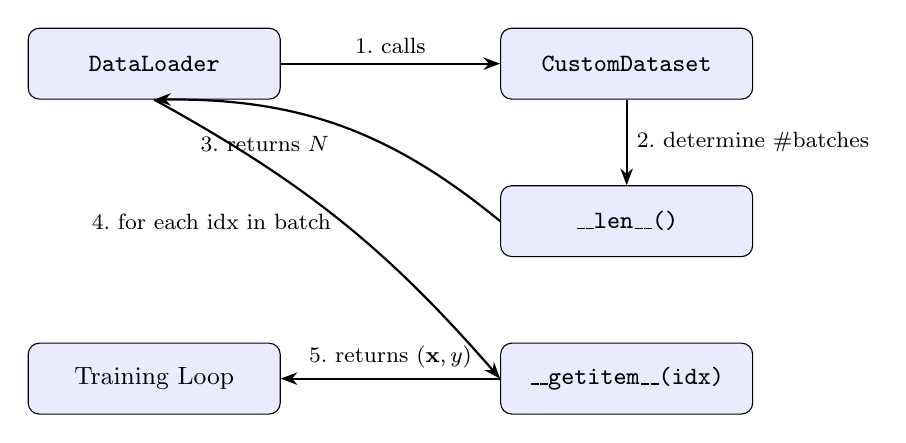
\begin{tikzpicture}[
  box/.style={rectangle, draw, rounded corners=4pt,
              minimum width=3.2cm, minimum height=0.9cm,
              fill=blue!8, font=\small},
  arrow/.style={-{Stealth[length=6pt]}, thick},
  note/.style={rectangle, draw=none, font=\footnotesize\itshape,
               text width=4cm, align=left}
]
  % Nodes
  \node[box] (dl)   at (0,0)    {\texttt{DataLoader}};
  \node[box] (ds)   at (6,0)    {\texttt{CustomDataset}};
  \node[box] (len)  at (6,-2)   {\texttt{\_\_len\_\_()}};
  \node[box] (gi)   at (6,-4)   {\texttt{\_\_getitem\_\_(idx)}};
  \node[box] (loop) at (0,-4)   {Training Loop};

  % Arrows
  \draw[arrow] (dl) -- node[above,font=\footnotesize]{1.\ calls} (ds);
  \draw[arrow] (ds) -- node[right,font=\footnotesize]{2.\ determine \#batches} (len);
  \draw[arrow] (len.west) to[bend right=20]
               node[below left,font=\footnotesize]{3.\ returns $N$} (dl.south);
  \draw[arrow] (dl.south) to[bend left=10]
               node[left,font=\footnotesize]{4.\ for each idx in batch} (gi.west);
  \draw[arrow] (gi) -- node[above,font=\footnotesize]{5.\ returns $(\mathbf{x},y)$} (loop);
\end{tikzpicture}
\caption{Call sequence between \texttt{DataLoader} and a custom \texttt{Dataset}.
The \texttt{DataLoader} first calls \texttt{\_\_len\_\_} to compute the number
of batches, then iteratively calls \texttt{\_\_getitem\_\_} to assemble each
batch tensor.}
\label{fig:dataset-dataloader}
\end{figure}

With $N = 4800$ and $B = 32$:
\begin{equation}
  \text{batches per epoch} = \left\lceil \frac{4800}{32} \right\rceil = 150
  \label{eq:batches}
\end{equation}

%% ============================================================
\section{Fashion-MNIST Dataset}
\label{sec:fashionmnist}
%% ============================================================

\subsection{Overview}
\label{subsec:fashionmnist-overview}

Fashion-MNIST is a dataset of grey-scale clothing images developed by Zalando
Research as a direct drop-in replacement for the classic handwritten-digit
MNIST dataset, but considerably more challenging.

\begin{table}[htbp]
  \centering
  \caption{Fashion-MNIST dataset properties}
  \label{tab:fashionmnist}
  \begin{tabular}{ll}
    \toprule
    \textbf{Property} & \textbf{Value} \\
    \midrule
    Image size          & $28 \times 28$ pixels \\
    Total pixels per image & $784$ \\
    Colour channels     & Grayscale (1 channel) \\
    Pixel value range   & 0 -- 255 (integer) \\
    Training samples    & 60{,}000 \\
    Test samples        & 10{,}000 \\
    Number of classes   & 10 \\
    Task type           & Multi-class classification \\
    Source              & Kaggle (\texttt{zalando-research/fashionmnist}) \\
    \bottomrule
  \end{tabular}
\end{table}

\subsection{Class Labels}
\label{subsec:class-labels}

Each image belongs to exactly one of the ten fashion categories listed in
\cref{tab:classes}.

\begin{table}[htbp]
  \centering
  \caption{Fashion-MNIST class labels}
  \label{tab:classes}
  \begin{tabular}{cl}
    \toprule
    \textbf{Label (integer)} & \textbf{Class name} \\
    \midrule
    0 & T-shirt / top \\
    1 & Trouser \\
    2 & Pullover \\
    3 & Dress \\
    4 & Coat \\
    5 & Sandal \\
    6 & Shirt \\
    7 & Sneaker \\
    8 & Bag \\
    9 & Ankle boot \\
    \bottomrule
  \end{tabular}
\end{table}

\subsection{ANN vs.\ CNN Representation}
\label{subsec:ann-vs-cnn}

The instructor explicitly highlights that this session uses the \emph{ANN
(fully connected)} approach, where each $28 \times 28$ image is
\emph{flattened} into a $784$-dimensional vector before being fed to the
network.  This loses spatial structure, which motivates the next topic:
Convolutional Neural Networks (CNNs), where the 2-D pixel grid is preserved.

\begin{keyinsight}[title=ANN vs.\ CNN on Image Data]
In an ANN for Fashion-MNIST:
\begin{itemize}
  \item The $28 \times 28$ image is flattened to a vector $\mathbf{x} \in \mathbb{R}^{784}$.
  \item All spatial relationships between neighbouring pixels are discarded.
  \item This is sufficient for simple benchmarks but sub-optimal for complex images.
\end{itemize}
CNNs (covered next) process the image as a 2-D grid, preserving local
spatial structure through convolutional filters.
\end{keyinsight}

\subsection{Data Preprocessing Pipeline}
\label{subsec:preprocessing}

The session uses a sample of 6{,}000 rows from the Kaggle \texttt{train.csv}
file (the full training set has 60{,}000 rows).  The preprocessing steps are:

\begin{enumerate}[label=\arabic*.]
  \item \textbf{Load CSV}: read 6{,}000 rows $\times$ 785 columns with
        \texttt{pandas.read\_csv}.  Column 0 is the label; columns
        1--784 are pixel values.
  \item \textbf{Split features and labels}: $\mathbf{X} = \text{df.iloc}[:,1:]$,
        $\mathbf{y} = \text{df.iloc}[:,0]$.
  \item \textbf{Train/test split}: 80\,\% train (4{,}800 rows),
        20\,\% test (1{,}200 rows) using \texttt{train\_test\_split}
        from scikit-learn.
  \item \textbf{Normalisation}: divide all pixel values by 255 so that
        $x_{ij} \in [0, 1]$.
  \item \textbf{Wrap in \texttt{CustomDataset}} and create
        \texttt{DataLoader} objects.
\end{enumerate}

The normalisation formula is:

\begin{equation}
  \tilde{x}_{ij} = \frac{x_{ij}}{255}, \quad x_{ij} \in \{0,\ldots,255\},
  \quad \tilde{x}_{ij} \in [0, 1]
  \label{eq:normalise}
\end{equation}

\begin{remark}
\label{rem:normalise}
Normalising pixel values to $[0,1]$ accelerates gradient-based optimisation
because features with large magnitudes produce large gradients, potentially
destabilising training.  Keeping all inputs in a common bounded range makes
the loss landscape better conditioned.
\end{remark}

%% ============================================================
\section{Neural Network Architecture}
\label{sec:architecture}
%% ============================================================

\subsection{Architecture Design}
\label{subsec:arch-design}

The target ANN for Fashion-MNIST classification has the following structure:

\begin{equation}
  784 \;\xrightarrow{\;\text{Linear}\;}\; 128
      \;\xrightarrow{\;\text{ReLU}\;}\;
      128 \;\xrightarrow{\;\text{Linear}\;}\; 64
      \;\xrightarrow{\;\text{ReLU}\;}\;
      64  \;\xrightarrow{\;\text{Linear}\;}\; 10
      \;\xrightarrow{\;\text{Softmax}\;}\; \hat{y}
  \label{eq:arch}
\end{equation}

Each layer performs a linear transformation followed by a non-linear
activation:

\begin{align}
  \mathbf{h}_1 &= \text{ReLU}(\mathbf{W}_1 \mathbf{x} + \mathbf{b}_1),
    \quad \mathbf{W}_1 \in \mathbb{R}^{128 \times 784},\;
          \mathbf{b}_1 \in \mathbb{R}^{128} \label{eq:layer1} \\
  \mathbf{h}_2 &= \text{ReLU}(\mathbf{W}_2 \mathbf{h}_1 + \mathbf{b}_2),
    \quad \mathbf{W}_2 \in \mathbb{R}^{64 \times 128},\;
          \mathbf{b}_2 \in \mathbb{R}^{64}  \label{eq:layer2} \\
  \mathbf{z}   &= \mathbf{W}_3 \mathbf{h}_2 + \mathbf{b}_3,
    \quad \mathbf{W}_3 \in \mathbb{R}^{10 \times 64},\;
          \mathbf{b}_3 \in \mathbb{R}^{10}   \label{eq:layer3} \\
  \hat{\mathbf{y}} &= \text{Softmax}(\mathbf{z}) \label{eq:softmax}
\end{align}

\subsection{TikZ Diagram of the ANN Architecture}
\label{subsec:arch-diagram}

\cref{fig:ann} shows the fully connected architecture.

\begin{figure}[htbp]
\centering
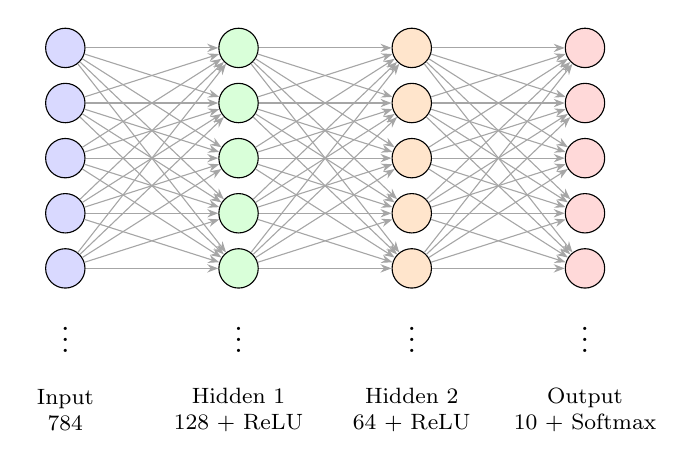
\begin{tikzpicture}[
  neuron/.style={circle, draw, fill=blue!15,
                 minimum size=0.5cm, inner sep=0pt},
  label_node/.style={rectangle, draw=none, font=\small\bfseries},
  arrow/.style={-{Stealth[length=4pt]}, gray!70, thin},
  layer_label/.style={font=\footnotesize, align=center}
]

% Column x-positions
\def\xIn{0}
\def\xH{2.2}
\def\xHH{4.4}
\def\xOut{6.6}

% Input layer (show 5 neurons + dots)
\foreach \i in {1,2,3,4,5}{
  \pgfmathsetmacro{\yy}{(\i-3)*0.7}
  \node[neuron] (I\i) at (\xIn,\yy) {};
}
\node[font=\large] at (\xIn,-2.2) {$\vdots$};

% Hidden layer 1 (show 5 neurons + dots)
\foreach \i in {1,2,3,4,5}{
  \pgfmathsetmacro{\yy}{(\i-3)*0.7}
  \node[neuron,fill=green!15] (H1\i) at (\xH,\yy) {};
}
\node[font=\large] at (\xH,-2.2) {$\vdots$};

% Hidden layer 2 (show 5 neurons + dots)
\foreach \i in {1,2,3,4,5}{
  \pgfmathsetmacro{\yy}{(\i-3)*0.7}
  \node[neuron,fill=orange!20] (H2\i) at (\xHH,\yy) {};
}
\node[font=\large] at (\xHH,-2.2) {$\vdots$};

% Output layer (show 5 neurons + dots)
\foreach \i in {1,2,3,4,5}{
  \pgfmathsetmacro{\yy}{(\i-3)*0.7}
  \node[neuron,fill=red!15] (O\i) at (\xOut,\yy) {};
}
\node[font=\large] at (\xOut,-2.2) {$\vdots$};

% Connections I->H1
\foreach \i in {1,2,3,4,5}{
  \foreach \j in {1,2,3,4,5}{
    \draw[arrow] (I\i) -- (H1\j);
  }
}

% Connections H1->H2
\foreach \i in {1,2,3,4,5}{
  \foreach \j in {1,2,3,4,5}{
    \draw[arrow] (H1\i) -- (H2\j);
  }
}

% Connections H2->O
\foreach \i in {1,2,3,4,5}{
  \foreach \j in {1,2,3,4,5}{
    \draw[arrow] (H2\i) -- (O\j);
  }
}

% Layer labels
\node[layer_label] at (\xIn,-3.2)  {Input\\784};
\node[layer_label] at (\xH,-3.2)   {Hidden 1\\128 + ReLU};
\node[layer_label] at (\xHH,-3.2)  {Hidden 2\\64 + ReLU};
\node[layer_label] at (\xOut,-3.2) {Output\\10 + Softmax};

\end{tikzpicture}
\caption{Fully connected ANN for Fashion-MNIST classification.
Inputs are the 784 normalised pixel values of a $28\times28$ greyscale image.
The two hidden layers use ReLU activation; Softmax is applied implicitly by
\texttt{nn.CrossEntropyLoss} during training.}
\label{fig:ann}
\end{figure}

\subsection{Activation Functions}
\label{subsec:activations}

\textbf{ReLU} (Rectified Linear Unit) is used in both hidden layers:
\begin{equation}
  \text{ReLU}(z) = \max(0, z)
  \label{eq:relu}
\end{equation}

\textbf{Softmax} converts raw output logits into a probability distribution
over the 10 classes:
\begin{equation}
  \text{Softmax}(z_k) = \frac{e^{z_k}}{\sum_{j=1}^{10} e^{z_j}},
  \quad k = 0, 1, \ldots, 9
  \label{eq:softmax-eq}
\end{equation}

\begin{remark}
\label{rem:softmax-in-loss}
In PyTorch, \texttt{nn.CrossEntropyLoss} combines the Softmax operation
with the negative log-likelihood loss.  Therefore it is \emph{not} necessary
(and is actually incorrect) to apply an explicit \texttt{nn.Softmax} layer
before the loss function.  The output of the final \texttt{nn.Linear} layer
(the raw logits $\mathbf{z}$) is passed directly to the loss.
\end{remark}

\subsection{Parameter Count}
\label{subsec:params}

The total number of learnable parameters is computed layer by layer.

\begin{table}[htbp]
  \centering
  \caption{Layer-wise parameter count for the $784 \to 128 \to 64 \to 10$ ANN}
  \label{tab:params}
  \begin{tabular}{lccr}
    \toprule
    \textbf{Layer} & \textbf{Input dim} & \textbf{Output dim} & \textbf{Parameters} \\
    \midrule
    Linear 1 (weights) & 784 & 128 & $784 \times 128 = 100{,}352$ \\
    Linear 1 (biases)  & --  & 128 & $128$ \\
    \textit{ReLU 1}    & 128 & 128 & $0$ \\
    Linear 2 (weights) & 128 & 64  & $128 \times 64 = 8{,}192$ \\
    Linear 2 (biases)  & --  & 64  & $64$ \\
    \textit{ReLU 2}    & 64  & 64  & $0$ \\
    Linear 3 (weights) & 64  & 10  & $64 \times 10 = 640$ \\
    Linear 3 (biases)  & --  & 10  & $10$ \\
    \midrule
    \textbf{Total} & & & \textbf{109,386} \\
    \bottomrule
  \end{tabular}
\end{table}

The dominant term is the first linear layer:
\begin{equation}
  \underbrace{784 \times 128}_{\text{weights}} + \underbrace{128}_{\text{biases}}
  = 100{,}480 \text{ parameters}
  \label{eq:first-layer-params}
\end{equation}

This accounts for $100{,}480 / 109{,}386 \approx 91.9\,\%$ of all learnable
parameters.

%% ============================================================
\section{nn.Module Implementation and Hands-On Walkthrough}
\label{sec:implementation}
%% ============================================================

\subsection{Toy nn.Module Example}
\label{subsec:toy-module}

Before building the full Fashion-MNIST model, the instructor demonstrates a
minimal \texttt{nn.Module} subclass to solidify the concept:

\begin{tcolorbox}[colback=gray!5!white, colframe=gray!60!black,
  fonttitle=\bfseries, title=Listing 3: Toy nn.Module (binary classification)]
\begin{verbatim}
import torch
import torch.nn as nn

class Model(nn.Module):
    def __init__(self, num_features):
        super().__init__()
        self.linear1  = nn.Linear(num_features, 3)
        self.relu     = nn.ReLU()
        self.linear2  = nn.Linear(3, 1)
        self.sigmoid  = nn.Sigmoid()

    def forward(self, features):
        out = self.linear1(features)
        out = self.relu(out)
        out = self.linear2(out)
        out = self.sigmoid(out)
        return out

# Usage
features = torch.rand(10, 5)          # 10 samples, 5 features
model    = Model(features.shape[1])   # num_features = 5
output   = model(features)            # calls forward()
# output shape: [10, 1]
\end{verbatim}
\end{tcolorbox}

\begin{example}[title=Two roles of nn.Module]
\begin{enumerate}[label=\arabic*.]
  \item \textbf{\texttt{\_\_init\_\_}}: Defines and registers all
        \emph{sub-modules} (layers). PyTorch tracks their parameters
        automatically for gradient computation.
  \item \textbf{\texttt{forward}}: Defines the computation graph,
        i.e.\ how data flows from input to output. Calling \texttt{model(x)}
        invokes \texttt{forward(x)} transparently.
\end{enumerate}
\end{example}

\subsection{MyNN: Full Fashion-MNIST Model}
\label{subsec:mynn}

The complete ANN used in the session is:

\begin{tcolorbox}[colback=gray!5!white, colframe=gray!60!black,
  fonttitle=\bfseries, title=Listing 4: MyNN -- Fashion-MNIST ANN]
\begin{verbatim}
class MyNN(nn.Module):
    def __init__(self, num_features):
        super().__init__()
        self.model = nn.Sequential(
            nn.Linear(num_features, 128),
            nn.ReLU(),
            nn.Linear(128, 64),
            nn.ReLU(),
            nn.Linear(64, 10)
            # No Softmax here: CrossEntropyLoss includes it
        )

    def forward(self, x):
        return self.model(x)
\end{verbatim}
\end{tcolorbox}

\subsection{nn.Sequential Container}
\label{subsec:sequential}

\texttt{nn.Sequential} chains modules in order.  The output of each module
automatically becomes the input of the next.  This models the mathematical
composition:

\begin{equation}
  f(\mathbf{x}) = \mathbf{W}_3 \cdot
    \text{ReLU}\!\left(\mathbf{W}_2 \cdot
      \text{ReLU}\!\left(\mathbf{W}_1 \mathbf{x} + \mathbf{b}_1\right)
      + \mathbf{b}_2\right)
    + \mathbf{b}_3
  \label{eq:sequential}
\end{equation}

\subsection{Loss Function and Optimiser}
\label{subsec:loss}

\begin{tcolorbox}[colback=gray!5!white, colframe=gray!60!black,
  fonttitle=\bfseries, title=Listing 5: Instantiating model, loss, and optimiser]
\begin{verbatim}
# Hyperparameters
num_epochs    = 100
learning_rate = 0.1

# Model
model     = MyNN(num_features=X_train.shape[1])

# Loss function (includes Softmax internally)
criterion = nn.CrossEntropyLoss()

# Optimiser: Stochastic Gradient Descent
optimizer = torch.optim.SGD(model.parameters(),
                            lr=learning_rate)
\end{verbatim}
\end{tcolorbox}

The cross-entropy loss for a single sample with true class $c$ and logit
vector $\mathbf{z}$ is:
\begin{equation}
  \mathcal{L}_{\text{CE}}(\mathbf{z}, c) =
  -\log\!\left(\frac{e^{z_c}}{\sum_{j=0}^{9} e^{z_j}}\right)
  = -z_c + \log\!\left(\sum_{j=0}^{9} e^{z_j}\right)
  \label{eq:ce-loss}
\end{equation}

\subsection{The Training Loop}
\label{subsec:training-loop}

\cref{alg:training} formalises the training procedure implemented in the
session notebook.

\begin{algorithm}[H]
\caption{Mini-Batch Training Loop for Fashion-MNIST ANN}
\label{alg:training}
\SetAlgoLined
\KwIn{train\_loader, model, criterion, optimizer, num\_epochs}
\KwOut{Trained model; epoch-level average loss printed each epoch}

\For{epoch $\leftarrow 1$ \KwTo \textup{num\_epochs}}{
  epoch\_loss $\leftarrow 0$ \;
  \For{(batch\_features, batch\_labels) \textbf{in} train\_loader}{
    \tcc{Step 1: Forward pass}
    outputs $\leftarrow$ model(batch\_features)\;
    \tcc{Step 2: Compute loss}
    loss $\leftarrow$ criterion(outputs, batch\_labels)\;
    \tcc{Step 3: Zero gradients, backward pass}
    optimizer.zero\_grad()\;
    loss.backward()\;
    \tcc{Step 4: Update parameters}
    optimizer.step()\;
    epoch\_loss $\leftarrow$ epoch\_loss $+$ loss.item()\;
  }
  avg\_loss $\leftarrow$ epoch\_loss $/ $ len(train\_loader)\;
  \textbf{print}(``Epoch'', epoch, ``Loss:'', avg\_loss)\;
}
\end{algorithm}

\begin{keyinsight}[title=The Four Steps of a Training Iteration]
Every mini-batch in every epoch executes exactly four operations:
\begin{enumerate}[label=\arabic*.]
  \item \textbf{Forward pass}: compute predictions $\hat{\mathbf{y}} = f(\mathbf{x}; \boldsymbol{\theta})$.
  \item \textbf{Loss computation}: evaluate $\mathcal{L}(\hat{\mathbf{y}}, \mathbf{y})$.
  \item \textbf{Backward pass}: compute $\nabla_{\boldsymbol{\theta}} \mathcal{L}$ via automatic differentiation.
  \item \textbf{Parameter update}: apply the SGD update rule (\cref{eq:sgd}).
\end{enumerate}
It is essential to call \texttt{optimizer.zero\_grad()} before
\texttt{loss.backward()} because PyTorch \emph{accumulates} gradients by
default across calls.
\end{keyinsight}

\subsection{Evaluation on the Test Set}
\label{subsec:evaluation}

After training, the model is switched to evaluation mode and accuracy is
computed:

\begin{tcolorbox}[colback=gray!5!white, colframe=gray!60!black,
  fonttitle=\bfseries, title=Listing 6: Test evaluation]
\begin{verbatim}
model.eval()
correct = 0
total   = 0

with torch.no_grad():
    for batch_features, batch_labels in test_loader:
        outputs    = model(batch_features)
        _, predicted = torch.max(outputs, dim=1)
        total   += batch_labels.size(0)
        correct += (predicted == batch_labels).sum().item()

accuracy = correct / total * 100
print(f"Test Accuracy: {accuracy:.2f}%")
\end{verbatim}
\end{tcolorbox}

The session reports a test accuracy of approximately \textbf{83\,\%} on the
1{,}200-sample test split (20\,\% of the 6{,}000-row sample dataset).

\begin{warningbox}[title=model.eval() is essential]
Calling \texttt{model.eval()} is not optional.  Certain layers (Dropout,
BatchNorm) behave differently during training versus inference.  Even if your
current architecture does not use these layers, it is best practice to always
set \texttt{model.eval()} before any inference or evaluation pass.  Pair it
with \texttt{torch.no\_grad()} to suppress gradient computation and reduce
memory usage.
\end{warningbox}

%% ============================================================
\section{torchinfo Model Summary}
\label{sec:torchinfo}
%% ============================================================

\subsection{Inspecting the Architecture with torchinfo}
\label{subsec:torchinfo}

The \texttt{torchinfo} library provides a Keras-style model summary for
PyTorch networks.  In the session:

\begin{tcolorbox}[colback=gray!5!white, colframe=gray!60!black,
  fonttitle=\bfseries, title=Listing 7: torchinfo summary call]
\begin{verbatim}
from torchinfo import summary
summary(model, input_size=(4800, 784))
\end{verbatim}
\end{tcolorbox}

The output (reproduced from the Colab notebook) is:

\begin{tcolorbox}[colback=black!5!white, colframe=black!40!white,
  fonttitle=\bfseries, title=torchinfo Output for MyNN]
\begin{verbatim}
=================================================================
Layer (type:depth-idx)    Output Shape        Param #
=================================================================
MyNN                      [4800, 10]          --
|-Sequential: 1-1         [4800, 10]          --
|  |-Linear: 2-1          [4800, 128]         100,480
|  |-ReLU: 2-2            [4800, 128]         --
|  |-Linear: 2-3          [4800, 64]          8,256
|  |-ReLU: 2-4            [4800, 64]          --
|  |-Linear: 2-5          [4800, 10]          650
=================================================================
Total params:             109,386
Trainable params:         109,386
Non-trainable params:     0
-----------------------------------------------------------------
Input size (MB):          15.05
Forward/backward size(MB):  7.76
Params size (MB):         0.44
=================================================================
\end{verbatim}
\end{tcolorbox}

\subsection{Verifying Parameter Counts}
\label{subsec:verify-params}

The \texttt{torchinfo} output can be verified analytically:

\begin{align}
  \text{Linear 1} &: 784 \times 128 + 128 = 100{,}480 \label{eq:p1} \\
  \text{Linear 2} &: 128 \times 64  + 64  = 8{,}256   \label{eq:p2} \\
  \text{Linear 3} &: 64  \times 10  + 10  = 650        \label{eq:p3} \\
  \text{Total}    &: 100{,}480 + 8{,}256 + 650 = 109{,}386 \label{eq:ptotal}
\end{align}

Note that \texttt{input\_size=(4800, 784)} specifies the full training set
shape for display purposes; the actual per-batch input shape during training
is $(32, 784)$.

%% ============================================================
\section{Complete Pipeline: Data Flow Diagram}
\label{sec:pipeline}
%% ============================================================

\cref{fig:pipeline} illustrates the complete end-to-end pipeline covered in
this session.

\begin{figure}[htbp]
\centering
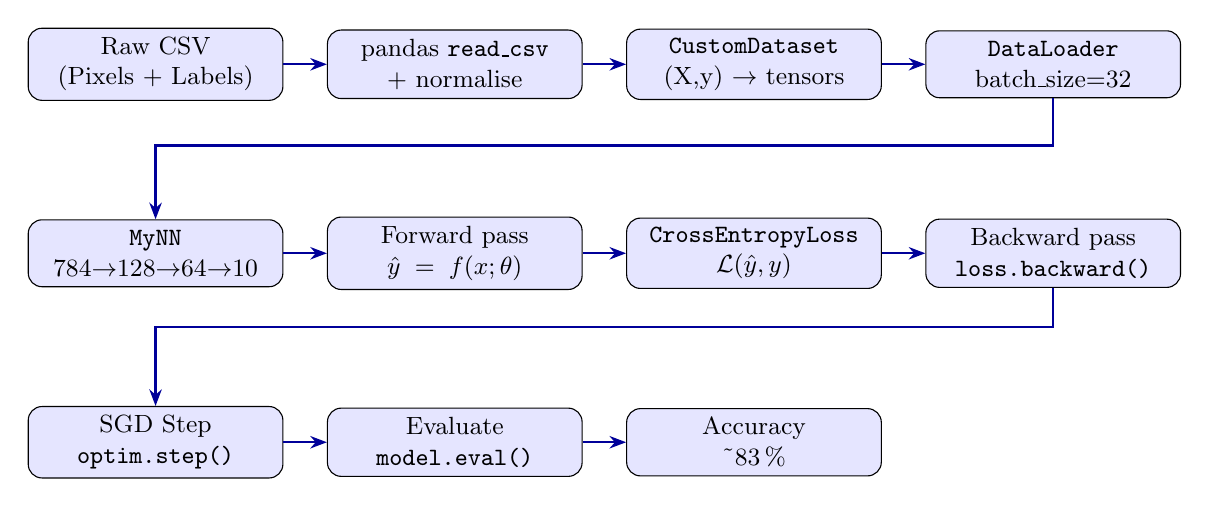
\begin{tikzpicture}[
  block/.style={rectangle, draw, rounded corners=5pt,
                fill=blue!10, minimum width=3.0cm,
                minimum height=0.85cm, font=\small,
                text centered, text width=3.0cm},
  decision/.style={diamond, draw, fill=yellow!15, font=\small,
                   text centered, aspect=2},
  arr/.style={-{Stealth[length=6pt]}, thick, blue!60!black},
  lab/.style={font=\footnotesize\itshape, midway}
]

\node[block] (raw)    at (0,0)     {Raw CSV\\(Pixels + Labels)};
\node[block] (pandas) at (3.8,0)   {pandas \texttt{read\_csv}\\+ normalise};
\node[block] (ds)     at (7.6,0)   {\texttt{CustomDataset}\\(X,y) $\to$ tensors};
\node[block] (dl)     at (11.4,0)  {\texttt{DataLoader}\\batch\_size=32};

\node[block] (model)  at (0,-2.4)  {\texttt{MyNN}\\$784{\to}128{\to}64{\to}10$};
\node[block] (fwd)    at (3.8,-2.4){Forward pass\\$\hat{y}=f(x;\theta)$};
\node[block] (loss)   at (7.6,-2.4){\texttt{CrossEntropyLoss}\\$\mathcal{L}(\hat{y},y)$};
\node[block] (bwd)    at (11.4,-2.4){Backward pass\\\texttt{loss.backward()}};

\node[block] (upd)    at (0,-4.8)  {SGD Step\\\texttt{optim.step()}};
\node[block] (eval)   at (3.8,-4.8){Evaluate\\\texttt{model.eval()}};
\node[block] (acc)    at (7.6,-4.8){Accuracy\\\textasciitilde83\,\%};

\draw[arr] (raw)    -- (pandas);
\draw[arr] (pandas) -- (ds);
\draw[arr] (ds)     -- (dl);
\draw[arr] (dl.south) -- ++(0,-0.6) -| (model.north);

\draw[arr] (model) -- (fwd);
\draw[arr] (fwd)   -- (loss);
\draw[arr] (loss)  -- (bwd);
\draw[arr] (bwd.south) -- ++(0,-0.5) -| (upd.north);

\draw[arr] (upd)  -- (eval);
\draw[arr] (eval) -- (acc);

\end{tikzpicture}
\caption{Complete end-to-end pipeline for Fashion-MNIST ANN training and
evaluation as implemented in Session~11.  The pipeline flows left to right,
then wraps to the next row.}
\label{fig:pipeline}
\end{figure}

%% ============================================================
\section{Q\&A Discussion Highlights}
\label{sec:qa}
%% ============================================================

Several important questions were raised during the session and are documented
here for completeness.

\subsection{Sigmoid vs.\ Softmax at the Output Layer}

\textbf{Question}: Do the neurons in this network use Sigmoid or Softmax?

\textbf{Answer}: Neither activation appears as an explicit \texttt{nn} module
in the model definition.  The hidden layers use ReLU.  The output layer
produces raw logits.  When \texttt{nn.CrossEntropyLoss} is called, it
internally applies Softmax and then computes the negative log-likelihood.  For
\emph{binary} classification, \texttt{nn.BCELoss} with a Sigmoid output would
be the appropriate choice.

The choice of output activation depends on the task type:
\begin{equation}
  \text{output activation} =
  \begin{cases}
    \text{Sigmoid} & \text{binary classification (2 classes)} \\
    \text{Softmax} & \text{multi-class classification ($>$2 classes)} \\
    \text{None (linear)} & \text{regression}
  \end{cases}
  \label{eq:activation-choice}
\end{equation}

\subsection{Streaming Data with DataLoader}

\textbf{Question}: Does PyTorch's \texttt{DataLoader} support streaming
(live) data feeds?

\textbf{Answer (instructor)}: The standard \texttt{DataLoader} is designed
for fixed-size datasets that can be indexed by integer position.  For
streaming scenarios (e.g.\ real-time sensor data), a custom iterable-style
\texttt{IterableDataset} subclass can be used, but this requires a different
implementation strategy.

\subsection{Gradient Zeroing -- Why Is It Necessary?}

\textbf{Question (implicit)}: Why is \texttt{optimizer.zero\_grad()} needed
before every backward pass?

\textbf{Answer}: PyTorch accumulates (adds) gradients to the
\texttt{.grad} attribute of each parameter tensor by default.  Without
zeroing, the gradient for batch $t$ would be the sum of all gradients from
batches $1, 2, \ldots, t$, which would corrupt the SGD update.

\begin{example}[title=Effect of not zeroing gradients]
Suppose the gradient of some weight $w$ is $+0.3$ in batch 1 and $-0.1$ in
batch 2.  Without zeroing, batch 2 would use $\nabla w = 0.3 + (-0.1) = +0.2$
instead of $-0.1$, giving an incorrect update direction.
\end{example}

\subsection{Building a Neural Network from Scratch}

\textbf{Question}: Is it possible to build a neural network without using
PyTorch?

\textbf{Answer}: Yes -- in the first weeks of the course the instructor
demonstrated manual implementation of forward propagation and gradient descent
using only NumPy, explicitly writing out $\mathbf{W}\mathbf{x} + \mathbf{b}$,
activation functions, and finite-difference gradient approximations.  PyTorch
automates the gradient computation (autograd), layer registration, and
optimisation steps that were done manually earlier.  The PyTorch abstraction
exists to make research and deployment tractable at scale.

%% ============================================================
\section{Summary and Conclusions}
\label{sec:summary}
%% ============================================================

\subsection{Key Concepts Covered}

Session~11 delivered a complete hands-on implementation cycle covering:

\begin{enumerate}[label=\arabic*.]
  \item \textbf{Dataset abstraction}: \texttt{CustomDataset(Dataset)} with
        \texttt{\_\_init\_\_}, \texttt{\_\_len\_\_}, and
        \texttt{\_\_getitem\_\_}.  The constructor converts raw arrays to
        typed tensors automatically on object creation.

  \item \textbf{DataLoader}: batches the dataset into mini-batches of size
        32 with shuffling for training data (to prevent class-sequential
        batches) and without shuffling for test data (for reproducibility).

  \item \textbf{Fashion-MNIST}: a benchmark of 70{,}000 $28\times28$
        greyscale clothing images across 10 classes; pixel values normalised
        to $[0,1]$.

  \item \textbf{ANN architecture} $784 \to 128 \to 64 \to 10$ with ReLU
        hidden activations and implicit Softmax via
        \texttt{nn.CrossEntropyLoss}; total 109{,}386 trainable parameters.

  \item \textbf{Training loop}: four-step mini-batch procedure (forward,
        loss, backward, update) repeated for 100 epochs $\times$ 150
        batches = 15{,}000 weight updates.

  \item \textbf{Evaluation}: test accuracy of $\approx 83\,\%$ on a
        1{,}200-sample hold-out set after training on 4{,}800 samples.

  \item \textbf{torchinfo}: layer-wise model inspection tool confirming
        output shapes and parameter counts.
\end{enumerate}

\subsection{What Comes Next}

The session closes with a preview of upcoming topics:

\begin{itemize}
  \item \textbf{CNN} (Convolutional Neural Network): the same Fashion-MNIST
        dataset will be revisited using convolutional layers that preserve
        the 2-D spatial structure of the image rather than flattening it.
  \item \textbf{Dropout and Batch Normalisation}: the significance of
        \texttt{model.eval()} vs.\ \texttt{model.train()} will be explored
        in detail when these regularisation layers are introduced.
  \item \textbf{Larger datasets}: using \texttt{torchvision.datasets} to
        load the full 60{,}000-sample version of Fashion-MNIST directly
        without downloading a CSV from Kaggle.
\end{itemize}

\subsection{Comparison: ANN vs.\ CNN for Image Classification}

\begin{table}[htbp]
  \centering
  \caption{Comparison of ANN and CNN approaches for Fashion-MNIST}
  \label{tab:ann-vs-cnn}
  \begin{tabularx}{\linewidth}{lXX}
    \toprule
    \textbf{Aspect} & \textbf{ANN (Session 11)} & \textbf{CNN (upcoming)} \\
    \midrule
    Input format & Flattened vector $\mathbb{R}^{784}$ &
      2-D grid $\mathbb{R}^{1 \times 28 \times 28}$ \\
    Spatial structure & Discarded & Preserved via conv.\ filters \\
    Parameters & 109{,}386 (dense) &
      Fewer (shared filter weights) \\
    Typical accuracy & $\approx 83\text{--}87\,\%$ &
      $\approx 90\text{--}94\,\%$ \\
    Key layers & \texttt{nn.Linear}, \texttt{nn.ReLU} &
      \texttt{nn.Conv2d}, \texttt{nn.MaxPool2d}, \texttt{nn.Linear} \\
    \bottomrule
  \end{tabularx}
\end{table}

\begin{keyinsight}[title=Core Takeaway]
The Dataset--DataLoader--Model--TrainingLoop pattern introduced in this
session is \emph{universal}.  Regardless of whether the model is an ANN, CNN,
RNN, or Transformer, the same four-step training loop and the same
Dataset/DataLoader infrastructure apply.  Mastering this pattern is the
foundation for all subsequent deep learning work in PyTorch.
\end{keyinsight}

\end{document}
